\documentclass[10pt]{article}

\usepackage[margin=1in]{geometry}
\usepackage[utf8]{inputenc}
\usepackage[T1]{fontenc}
\usepackage{amsmath,amssymb,amsthm}
\usepackage{graphicx}
\usepackage{booktabs}
\usepackage{listings}
\usepackage{xcolor}
\usepackage[colorlinks=true,linkcolor=blue,citecolor=blue,urlcolor=blue]{hyperref}
\usepackage{natbib}

% --- Lean code listing style ---
\lstdefinelanguage{lean}{
  morekeywords={class, def, theorem, instance, where, by, induction, with, intro, rw, exact, simp, ext, fin\_cases, dsimp, unfold, variable, namespace, end, import, open, structure, extends, cases, refine, obtain},
  sensitive=true,
  morecomment=[l]{--},
  morestring=[b]",
}
\lstset{
  language=lean,
  basicstyle=\ttfamily\small,
  keywordstyle=\color{blue!70!black}\bfseries,
  commentstyle=\color{gray},
  breaklines=true,
  columns=fullflexible,
  frame=single,
  framesep=3pt,
  xleftmargin=3pt,
  xrightmargin=3pt,
}

\newtheorem{theorem}{Theorem}[section]
\newtheorem{remark}[theorem]{Remark}

% Float placement: the default \textfraction of 0.2 forbids a page from being
% more than 80% float, which with seven listings, six tables and three figures
% pushed floats forward and left whitespace behind them. Relaxing the fractions
% packs floats beside text instead of onto near-empty pages. Typesetting only --
% no content is affected.
\renewcommand{\topfraction}{0.92}
\renewcommand{\bottomfraction}{0.85}
\renewcommand{\textfraction}{0.06}
\renewcommand{\floatpagefraction}{0.80}
\setcounter{topnumber}{3}
\setcounter{bottomnumber}{2}
\setcounter{totalnumber}{5}

\emergencystretch=2em

\title{\textbf{Necessary but Not Sufficient:\\ What Non-Commutative Binding Buys in Vector-Symbolic Architectures}}

\author{
  Vu Linh Nguyen-Van\thanks{Corresponding author.} \quad Thai Son Nguyen \quad Bao-An Nguyen \\
  \small Tra Vinh University, Tra Vinh, Vietnam \\
  \small \texttt{vlinhd11@tvu.edu.vn}, \texttt{thaison@tvu.edu.vn}, \texttt{annb@tvu.edu.vn}
}
\date{}

\begin{document}
\maketitle

\begin{abstract}
Vector-symbolic architectures choose non-commutative binding when they need ordered structure. We ask what that choice actually buys, and answer with machine-checked theorems in Lean 4. Order sensitivity is not a property of the binding matrix but of the \emph{label algebra} whose action it realizes, so an abelian one is excluded by inspection --- any carrier, any label type. That criterion separates four requirements the field treats as one. Ordered pairs need two distinct roles, which a commutative operator supplies. Chain recovery needs a left inverse, which a commutative operator has. Reordering is where non-commutativity is genuinely necessary: if labels commute, every permutation of a chain is the same map, at every length. But it is \emph{not sufficient} for direction, and this is the result we did not expect: our own verified operator family satisfies the order axiom and is blind to reversal at every odd chain length --- machine-checked at length three, exhaustive over all words at five and seven --- because it exposes two of its group's eight elements. Exposing all eight repairs it, with a distinguishing chain at every length. Measured on real curriculum hop lengths, the two commutative arms are reversal-blind at 33 of 33 lengths, the two-generator family at exactly the 16 odd ones, and the family exposing all eight at none. What binds a system is therefore not non-commutativity but how much of its label algebra it uses.
\end{abstract}

\section{Introduction}
\label{sec:intro}

Vector-symbolic architectures (VSAs), also called hyperdimensional computing, represent structured knowledge as fixed-width hypervectors combined by binding, bundling and permutation \citep{kanerva2009hyperdimensional,kleyko2022survey}. They fit a specific shape of problem: a fixed-width state, updated in $O(1)$ with no backpropagation, holding an arbitrarily long ordered sequence and recovering a position along it exactly. Ordered prerequisite structure has that shape --- the curriculum graph used throughout has 971 direct edges inducing 56{,}224 transitive relations, 85.2\% of them spanning seven hops or more, so what a curriculum encodes is overwhelmingly long-range and what a learner traverses is a path, not an edge.

Which algebraic property does that require? The field answers \emph{non-commutativity}. Holographic reduced representations, matrix binding and block-diagonal rotation constructions are chosen for ordered composition precisely because, unlike commutative alternatives such as Multiply-Add-Permute (MAP), they can in principle distinguish the order in which things are combined \citep{plate1995holographic,gayler1998connections,gallant2013mbat,schlegel2022comparison}. PathHD lists an ``order-sensitive, non-commutative binding operator'' as its first technical component and validates the resulting system by Hits@1 \citep{liu2025pathhd}; quaternion knowledge-graph embeddings adopt quaternions in part because quaternion multiplication does not commute \citep{zhang2019quate}. The property is rarely checked directly; it is checked by whether a downstream classifier works.

We check it directly, over the specification fixed in \S\ref{sec:prelim}. The organizing result is a criterion rather than a catalogue: order sensitivity is not a property of the binding matrix but of the \emph{label algebra} whose action the matrix realizes. Composing two binds lands back inside the family, at the composite relation label, and presenting a family that way moves the question from the carrier to the label algebra --- where the answer is clean. No family that is the action of an \emph{abelian} label algebra can satisfy an intra-family order-sensitivity axiom, for any carrier, any label type, and any transformations (Theorem~\ref{thm:abelian}), so an operator can be placed by inspecting how its labels compose.

That criterion separates four requirements the literature collapses into one word. An ordered \emph{pair} needs two distinct roles, and two \emph{commutative} roles already suffice (\S\ref{sec:pairs}). \emph{Recovery} of a composed chain needs a left inverse and nothing else, so a commutative operator achieves it, and we measure it (\S\ref{sec:recovery}). \emph{Reordering} is where the axiom is genuinely load-bearing, in both directions: if labels commute, every permutation of a chain acts identically at every length (Theorem~\ref{thm:perm}), and conversely the axiom yields two orderings that differ, at every length (Theorem~\ref{thm:order-general}).

The fourth requirement is where we were wrong, and it is the result of this paper. \emph{Direction} --- telling a traversal from its reverse, which is what prerequisite structure turns on --- is one particular reordering, and the axiom does not deliver it. Our own verified integer family satisfies the axiom and is provably blind to reversal at chain length three, with exhaustive search finding the same at every odd length (Theorem~\ref{thm:blind}); the cause is not the axiom but the family, which exposes two of its group's eight elements. Exposing all eight yields a distinguishing chain at every length (Theorem~\ref{thm:d4}). Two families, both satisfying the same axiom, differing in whether they can represent direction at all.

All of it is measured on the quantity the theorems are about --- forward composition, no unbinding (\S\ref{sec:order-exp}). On real curriculum hop lengths the two commutative arms are reversal-blind at 33 of 33 lengths, the two-generator family at exactly the 16 odd ones, and the family exposing all eight at none: a categorical split, and the only place in this paper where the arms separate rather than tie. The remaining cost, superposition, is measured against a law whose exponent we fit rather than assume (\S\ref{sec:capacity-exp}).

\paragraph{Contributions.} (i) A criterion for placing a binding operator, locating order sensitivity in the label algebra so that an operator can be positioned without a per-instance proof (\S\ref{sec:criterion}, Table~\ref{tab:criterion}). (ii) A separation of four requirements the field treats as one, with the price of each stated and machine-checked (\S\ref{sec:pairs}--\ref{sec:direction}). (iii) The finding that non-commutativity is \emph{not sufficient} for direction, with a counterexample inside our own verified family, an algebraic repair, and a runtime signature that separates the two on real curriculum hop lengths (\S\ref{sec:direction}, \S\ref{sec:order-exp}). (iv) A machine-checked artifact reported as data (\S\ref{sec:artifact}), and measurements on the theorems' own quantity, including a closed-form prediction for the two-hop case confirmed against measurement, a superposition exponent fitted at $0.48$ against a predicted $0.5$, and five settings in which the operator provably cannot matter and measurably does not.


\section{Related Work}
\label{sec:related}

\paragraph{Binding operators and order.} \citet{kanerva1988sparse} established that fixed-width random hypervectors support robust associative storage; \citet{kanerva1996binary} developed binary spatter-coding for ordered $k$-tuples; \citet{kanerva2009hyperdimensional} consolidated the paradigm; \citet{plate1995holographic,plate2003holographic} constructed circular-convolution binding with bounded capacity; \citet{gayler1998connections} analysed binding and unification as competing design pressures. Two later operators are non-commutative by design and are the closest precedents for the family we verify: \citet{gallant2013mbat} bind with a \emph{matrix} acting on additive terms, and \citet{gosmann2019vtb} derive a transformation binding with better fixed-point behaviour than convolution. \citet{schlegel2022comparison} survey the landscape and tabulate exactly the properties at issue here --- commutativity, invertibility, self-inverseness --- across MAP, HRR, BSC, VTB and MBAT; that table is the clearest statement of the assumption this paper examines.

\paragraph{Order without a non-commutative bind.} The field's other answer to order is permutation: a fixed $\rho$ applied $k$ times marks position $k$, so an ordered sequence is representable with a commutative bind \citep{kanerva1996binary,kleyko2022survey}. Our criterion covers that case rather than competing with it. A family generated by a single $\rho$ is the action of a cyclic --- hence \emph{abelian} --- label algebra, so Theorem~\ref{thm:abelian} excludes it intra-family and Theorem~\ref{thm:perm} makes a chain of such binds invariant under reordering. Permutation encoding evades this by putting position in the \emph{exponent} rather than in the composition order: a different representational choice with a different cost, not a counterexample, and not one that makes composition order-sensitive.

\paragraph{Non-commutativity in knowledge-graph embeddings.} \citet{sun2019rotate} designed RotatE, composing a relation with an entity by the Hadamard product of unit-modulus complex vectors, and proved it can represent antisymmetric relations. Two features bear on us: the property established is asymmetry of a relation under inversion, not order sensitivity of composition; and the composition operator itself is commutative, since composing two relations adds their phases. The second point is machine-checked rather than interpretive --- \texttt{no\_additive\_label\_PedagogicalVSA} (\S\ref{sec:criterion}) shows no family whose labels compose by addition can satisfy the axiom, whatever the carrier and whatever the individual rotations do. \citet{zhang2019quate} go further and adopt quaternions, whose multiplication does not commute; that is the strongest instance of the belief we examine, a design chosen \emph{because} the algebra is non-commutative. \S\ref{sec:direction} is the caution that applies to it: non-commutativity of the ambient algebra does not by itself let a model distinguish a composition from its reverse, since that depends on which elements the learned relations occupy.

\paragraph{Verification, capacity, and educational structure.} \citet{demoura2021lean4} developed Lean 4 and \citet{mathlib2020} its mathematical library. \citet{shaw2025category} gave a category-theoretic foundation for VSA algebra without machine-checking the axioms. Most closely related, \citet{scott2026avsad} couple an LLM ensemble with Lean 4 property-testing to \emph{discover} binding operators satisfying associativity and non-commutativity; those properties are agnostic to any particular pair of vectors and do not imply exact unbinding, and our difference is not only a stronger property but a different question --- they ask which operators are non-commutative, we ask what non-commutativity is for. On capacity, \citet{frady2017superposition,frady2018theory} analyse retrieval from a superposition of $M$ items in $N$ dimensions and show accuracy depends on the ratio alone, with signal-to-noise $\sqrt{N/M}$, independently of the moments of the code distribution --- their explanation for a channel capacity of roughly half a bit per neuron shared across VSA models --- and \citet{thomas2021hd} give a complementary account of the same regime; \citet{kumar2026holographic} localizes the failure of zero-shot two-hop composition to that bottleneck, explicitly exonerating the bind/unbind algebra. On educational structure, \citet{corbett1994knowledge} introduced Bayesian Knowledge Tracing and \citet{piech2015deep} replaced its hidden Markov model with a recurrent network; \citet{liu2025pathhd} encode relational paths with the block-diagonal family that motivates our operator; \citet{zou2025metacog} used HDC binding for meta-level self-monitoring and \citet{girard2026counterfactual} framed instructional policy selection as a contextual bandit; and on prerequisite learning, \citet{zhou2024psikt} jointly infer learner traits and a prerequisite graph while directed-graph methods treat prerequisite direction as a learned embedding property \citep{qu2024cprp,zhang2025gkrom,zhang2025dgcpl,cheng2026proprl}.


\section{Preliminaries}
\label{sec:prelim}

\paragraph{Notation.} Fix a carrier type $V$. A binding \emph{family} maps relation indices $i \in \mathbb{N}$ to transformations $\texttt{ops}\ i : V \to V$ with matching left inverses $\texttt{inv}\ i$. Superposition is $\texttt{bundle} : V \to V \to V$. We reserve $u,v$ for concept representations, $Y$ for an arbitrary carrier element, $i,j$ for relation indices, $n$ for chain length, $D$ for hypervector dimension, and $T$ for superposition load. In the kernel tier the carrier is \texttt{Matrix2 Int}, the $2\times2$ integer matrices, with \texttt{add} for superposition and matrix multiplication for binding; \texttt{zero2} is the zero matrix and \texttt{Matrix2.one} the identity. Two transformations recur: \texttt{Rot}, the $90^\circ$ rotation, and \texttt{Ref}, a reflection.

\paragraph{The specification.} A VSA over $V$ is a family of binding operations with matching left inverses, a bundling operation, and three axioms (\texttt{src/eduhdc/\allowbreak EduBindSelfContained.lean}; Unicode connectives are transliterated and doc comments condensed for space, here and in every listing):

\begin{lstlisting}
structure PedagogicalVSA (V : Type) where
  bundle : V -> V -> V
  ops : Nat -> (V -> V)
  inv : Nat -> (V -> V)
  exact_unbind_ax : forall i Y, inv i (ops i Y) = Y
  bundle_distrib_ax : forall i X Y, ops i (bundle X Y) = bundle (ops i X) (ops i Y)
  order_sensitive_ax : exists i j Y, ops i (ops j Y) != ops j (ops i Y)
\end{lstlisting}

We call these Axiom 1 (distributivity of binding over superposition), Axiom 2 (order sensitivity), and Axiom 3 (exact unbinding). A curriculum contains many relations, so the object specified is a \emph{family}, and Axiom 2 is quantified over two members of that family rather than over a second, free binding operation. That choice is load-bearing: a provably commutative elementwise binding satisfies Axioms 1 and 3, and under a free-second-operation formulation would satisfy Axiom 2 as well, since for almost any invertible binding \emph{some} unrelated map fails to commute with it.

Two scope notes. \texttt{exact\_unbind\_ax} is a left-inverse law, so binding need not be surjective; a strengthened two-sided contract is separately discharged for both integer instances, so nothing below depends on the weaker form. And \texttt{bundle} carries no axioms beyond distributivity --- \S\ref{sec:pairs} turns that gap into a result rather than leaving it a caveat.

\section{Order Sensitivity Lives in the Label Algebra}
\label{sec:criterion}

Axiom 2 has content only if some families provably fail it, and both concrete impossibility results are instances of one fact about where order sensitivity lives. Composing two binds lands back inside the family, at the composite label; presenting a family that way --- as the action of a label algebra $G$ on the carrier --- moves Axiom 2 from the carrier to the label algebra (\texttt{src/eduhdc/\allowbreak GroupActionSpec.lean}):

\begin{lstlisting}
structure ActionFamily (G : Type) (V : Type) where
  act : G -> (V -> V)
  comp : G -> G -> G
  act_comp : forall g h Y, act g (act h Y) = act (comp g h) Y
\end{lstlisting}

\begin{theorem}[\texttt{no\_abelian\_action\_PedagogicalVSA}]
\label{thm:abelian}
No binding family that is the action of an \emph{abelian} label algebra can satisfy Axiom 2 --- for any carrier, any label type, and any choice of transformations.
\end{theorem}

\begin{lstlisting}
theorem no_abelian_action_PedagogicalVSA
    {G V : Type} (P : PedagogicalVSA V) (A : ActionFamily G V) (gen : Nat -> G)
    (hab : forall g h, A.comp g h = A.comp h g)
    (hops : forall i, P.ops i = A.act (gen i)) : False := by
  obtain <i, j, Y, hne> := P.order_sensitive_ax
  rw [hops i, hops j] at hne
  exact hne (A.commutes_of_abelian hab (gen i) (gen j) Y)
\end{lstlisting}

\emph{Proof.} If labels commute then the transformations commute pointwise, by rewriting along \texttt{act\_comp} twice; Axiom 2 asserts a pair that does not. No property of the carrier is consulted. $\blacksquare$

\begin{remark}
\label{rem:criterion}
The proof is three lines, and that is the point rather than a concession: the content is in the \emph{presentation}, not the argument. One hypothesis excludes an infinite class at once --- every elementwise family whatever its matrices, every additive-phase family whatever its angles --- where a per-family proof settles one construction at a time. Two limits follow, neither hidden below: the condition is necessary but not sufficient, since Axioms 1 and 3 separately demand linearity and invertible action, and it constrains only families closed under composition, which the \texttt{ops} field of \texttt{PedagogicalVSA} does not require.
\end{remark}

\begin{table}[t]
\centering
\caption{Applying the criterion. Membership requires a non-abelian label algebra (Theorem~\ref{thm:abelian}); the exclusions follow from the second column. Three are discharged by a named Lean theorem; circular convolution and single-generator permutation are excluded by the same argument applied to their label algebras, which we state rather than mechanize separately. The two commutative arms measured in \S\ref{sec:experiments} are excluded on this ground, not only empirically.}
\label{tab:criterion}
\small
\begin{tabular}{llp{0.33\textwidth}}
\toprule
Binding operator & Labels compose by & Verdict \\
\midrule
Elementwise (MAP, Hadamard)        & elementwise product, abelian & excluded, \texttt{no\_hadamard\_\allowbreak via\_action} (checked) \\
Circular convolution (HRR)         & convolution, abelian         & excluded by Theorem~\ref{thm:abelian}, by inspection \\
Additive phase (RotatE-style)      & addition, abelian            & excluded, \texttt{no\_additive\_\allowbreak label\_\allowbreak PedagogicalVSA} (checked) \\
Rotations only ($SO(2)$)           & angle addition, abelian      & excluded, \texttt{no\_rotation\_\allowbreak only\_\allowbreak PedagogicalVSA} (checked) \\
Powers of one permutation $\rho$   & cyclic, abelian              & excluded by Theorem~\ref{thm:abelian}, by inspection \\
Integer $O(2)$, signed permutation & matrix product, non-abelian  & admitted, two verified instances \\
Dihedral labels, $G \neq V$        & dihedral rule, non-abelian   & admitted, \texttt{d4VSA} (\S\ref{sec:direction}) \\
Real $O(3)$, block-diagonal, $U(2)$ & matrix product, non-abelian & admitted, \texttt{ofOrthogonalFamily}, \texttt{ofUnitaryFamily} \\
\bottomrule
\end{tabular}
\end{table}

The first row is a corollary rather than a separate fact. Elementwise binding is the action of $2\times2$ integer matrices composing elementwise, abelian because integer multiplication is, so no family drawn entirely from it can satisfy Axiom 2, for any choice of matrices. \texttt{no\_hadamard\_via\_action} is correspondingly one line: it applies Theorem~\ref{thm:abelian} to the elementwise action, with no argument of its own. Remark~\ref{rem:criterion} states what the criterion does and does not settle. A second, directly proved version generalizes differently: \texttt{no\_hadamard\_PedagogicalVSA\_comm} consumes only commutativity and associativity of multiplication, so it transfers to any carrier providing those two laws. The rotation-only row is proved over real matrices in the Mathlib tier, and is why the family we verify is the full orthogonal group $O(2)$ rather than $SO(2)$.

The two concrete impossibility theorems carry a scope limit: they rule out families drawn \emph{entirely} from the named construction, not mixed families containing one order-sensitive pair. A strengthened axiom quantified over every pair of operators that differ as functions closes that loophole and is discharged for both integer instances (\texttt{PedagogicalVSAStrong}), though not for a family large enough to exercise the mixed case.

\paragraph{Instances.} On the integer carrier, binding by an integer point of $O(2)$ and by signed permutation both satisfy the specification; in dimension two those groups coincide, so we claim two verified instances rather than two independent operators. Among admissible label algebras $O(2)$ is the cheapest we know of, its inverse being the transpose at the cost of a sign flip, measured in \S\ref{sec:pair-tiers} at exact fp32 recovery and $0.9998$ cosine fidelity under int8. Over the reals, \texttt{ofOrthogonalFamily} admits any family of orthogonal real matrices, over any finite index type, non-commuting at one pair; it is discharged at $3\times3$ --- a pair of quarter turns generating a non-abelian subgroup of $SO(3)$ --- and at block-diagonal matrices with orthogonal blocks at any block count, and \texttt{ofUnitaryFamily} is the same argument at the conjugate transpose, discharged at a block-diagonal $U(2)$ carrier.

\section{Pairs: Two Commutative Roles Suffice}
\label{sec:pairs}

Axiom 2 constrains the \emph{composition} of two binds on one content vector. The motivating requirement concerns an ordered \emph{pair} of concepts. Nothing so far connects them, and this section finds the connection weaker than expected in one direction and unnecessary in the other (\texttt{src/eduhdc/\allowbreak EncPairSpec.lean}). We use the standard role-filler encoding, $\texttt{encPair}\ i\ j\ u\ v = \texttt{bundle}\,(\texttt{ops}\ i\ u)\,(\texttt{ops}\ j\ v)$: bind $u$ to one role, $v$ to another, superpose.

\begin{theorem}[\texttt{encPair\_axioms\_insufficient}]
\label{thm:insufficient}
There is a \texttt{PedagogicalVSA} instance whose \texttt{ops} family is order-sensitive and whose pair encoding is nevertheless order-blind: \texttt{encPair} takes the same value on $(u,v)$ and $(v,u)$, for every content and every pair of roles.
\end{theorem}

\emph{Proof.} The witness \texttt{edubindCollapsedBundle} reuses the verified family's own \texttt{ops} and \texttt{inv} --- so Axioms 2 and 3, which never mention \texttt{bundle}, are inherited unchanged --- and replaces \texttt{bundle} by a constant function. Axiom 1 holds because every family member fixes the zero matrix. The instance is genuine, and its pair encoding is constant. $\blacksquare$

Theorem~\ref{thm:insufficient} is a refutation, not an unproved gap, and it locates the missing ingredient: \texttt{bundle} carries no axiom preventing it from erasing its arguments. The witness is deliberately degenerate, and that is the point --- the axioms do not exclude it, so they cannot be what makes a pair encoding work. Adding a bundle identity that every operator fixes restores the property: under \texttt{PedagogicalVSAPointed} the encoding is order-sensitive at $(Z, \texttt{zero})$ exactly when the two operators disagree pointwise at $Z$, discharged for both integer instances.

\subsection{Two commutative roles are already enough}
\label{sec:h0}

The sharper result is that the pair encoding does not need the order-sensitivity axiom at all.

\begin{theorem}[\texttt{hadamard\_encPair\_order\_sensitive\_bipolar}]
\label{thm:h0}
The role-filler pair encoding built on elementwise binding is order-sensitive, with roles and contents that are \emph{legal elementwise codebook entries}: all four are bipolar and each is its own Hadamard inverse. This holds for a family that provably cannot satisfy Axiom 2 (Table~\ref{tab:criterion}, row 1), and involves no composition of two binds anywhere.
\end{theorem}

The Lean statement, \texttt{hadamard\_encPair\_order\_sensitive\_bipolar}, asks for four matrices each of which squares elementwise to the all-ones matrix --- the identity for elementwise binding, not \texttt{Matrix2.one} --- together with $\texttt{encPairHad}\ M\ N\ u\ v \neq \texttt{encPairHad}\ M\ N\ v\ u$, where $\texttt{encPairHad}\ M\ N\ u\ v = (M \odot u) + (N \odot v)$.

\emph{Proof.} Take $M = u = (1,1,1,1)$ and $N = v = (1,-1,1,-1)$, each its own Hadamard inverse and so a legal role or content. The $a_{01}$ entry of $\texttt{encPairHad}\ M\ N\ u\ v$ is $1{\cdot}1 + (-1){\cdot}(-1) = 2$; of $\texttt{encPairHad}\ M\ N\ v\ u$ it is $1{\cdot}(-1) + (-1){\cdot}1 = -2$. Closed by \texttt{omega} after one field projection. $\blacksquare$

An earlier version of this witness used a role that is not invertible over the integers: the theorem was true, but the witness did not lie in the family it stood for, while the commutative arm measured in \S\ref{sec:pair-tiers} draws from a bipolar codebook. The statement is existential, the correct form for refuting a necessity claim, and does not assert that every elementwise encoding distinguishes order. Theorem~\ref{thm:abelian} widens what the witness stands for: the family is excluded not by any property of elementwise multiplication but by abelian label composition, while the encoding uses only two distinct roles and a bundle, neither of which touches how labels compose. The construction therefore transfers to any abelian-label binding, phase composition included --- a reading of the two theorems together rather than a third theorem.

\begin{remark}
\label{rem:predictions}
Theorem~\ref{thm:h0} suggests a testable expectation, taken up in \S\ref{sec:pair-tiers}: on a benchmark whose task reduces to pair-level order recovery, a commutative binding and an order-sensitive non-VSA encoding should both be able to match a verified non-commutative operator. The theorem is existential, so this is an expectation rather than an entailment. Five independent settings turn out consistent with it.
\end{remark}

\section{Recovery Needs Only a Left Inverse}
\label{sec:recovery}

A single exact bind/unbind pair guarantees nothing about a \emph{chain}. Two things close that gap: induction on length, and the fact that a real chain traverses a \emph{different} relation at every hop, so the roundtrip is indexed by a sequence of relations rather than a repetition count (\texttt{src/eduhdc/\allowbreak ChainTransitivity.lean}). \texttt{chainRoundtrip} is two lines: the empty chain is the identity, and $i :: \texttt{is}$ binds by $\texttt{ops}\ i$, recurses on the tail, and unbinds by $\texttt{inv}\ i$. \texttt{chain\_exact\_unbind} is then a four-line induction on the list, the base case by reflexivity and the step by the inductive hypothesis followed by \texttt{exact\_unbind\_ax}. For any instance, any relation list of any length, and any content, binding forward and unbinding back recovers the content exactly --- for every heterogeneous relation sequence, not as a statistic over sampled chains. Two things about it are easy to over-read, and both matter. The proof consumes exactly one axiom, \texttt{exact\_unbind\_ax}; it never mentions Axiom 2. So exact chain recovery is available to \emph{any} family with left inverses, including the abelian families Theorem~\ref{thm:abelian} excludes: elementwise binding satisfies $x \odot x = \mathbf{1}$ pointwise and therefore has one. Non-commutativity cannot be what buys chain recovery, and \S\ref{sec:capacity-exp} measures a commutative operator achieving it at every length up to 150. And \texttt{chainRoundtrip} calls \texttt{ops} and \texttt{inv} but \emph{never} \texttt{bundle}, at any length, so it holds one live value at a time --- the property \S\ref{sec:capacity-exp} contrasts with role-filler encoding.

\section{Reordering: Necessary}
\label{sec:reorder}

What an abelian family loses is the order itself, and two theorems isolate it (\texttt{src/eduhdc/\allowbreak ChainOrder.lean}). Both are stated over \texttt{chainOps} / \texttt{chainAct}, forward chain application in which \texttt{inv} never appears, so neither reads Axiom 3 and the order question is separable from the recovery one.

\begin{theorem}[\texttt{abelian\_chainAct\_perm}]
\label{thm:perm}
For any action family whose label algebra is abelian, any two chains that are permutations of one another act identically --- not merely a chain and its reverse --- at every length and with no invertibility assumed.
\end{theorem}

\begin{lstlisting}
theorem abelian_chainAct_perm (A : ActionFamily G V) (gen : Nat -> G)
    (hab : forall g h, A.comp g h = A.comp h g) :
    forall {is js : List Nat}, is.Perm js -> forall (Y : V),
      chainAct A gen is Y = chainAct A gen js Y := by
  intro is js hp
  induction hp with
  | nil => intro Y; rfl
  | cons x _ ih =>
    intro Y
    dsimp [chainAct]
    rw [ih Y]
  | swap x y l => intro Y; exact chainAct_swap_of_abelian A gen hab y x l Y
  | trans _ _ ih1 ih2 => intro Y; rw [ih1 Y, ih2 Y]
\end{lstlisting}

\emph{Proof.} One adjacent transposition is invisible to an abelian family, by \texttt{commutes\_of\_abelian} applied at the tail's value. \texttt{List.Perm} is generated by exactly that transposition together with \texttt{cons}, \texttt{trans} and \texttt{nil}, so induction on the permutation derivation closes every case. $\blacksquare$

The permutation form costs four lines more than the reversal form and is strictly stronger, so we state it as the theorem and take reversal as its instance; \texttt{hadamard\_chainAct\_perm} instantiates it at the concrete elementwise action, and that is what \S\ref{sec:order-exp} measures.

\paragraph{Where the negative direction may be stated.} The two halves of this section live over \emph{different} structures, and the asymmetry is forced. The positive half below lives over \texttt{PedagogicalVSA}, which has instances, so it is non-vacuous. The negative half must not: \texttt{PedagogicalVSA} carries Axiom 2, and Theorem~\ref{thm:abelian} derives $\bot$ from exactly the hypotheses such a statement would assume, so an order-blindness theorem stated there would type-check, keep \texttt{lake build} green, and be quantified over an empty domain. \texttt{abelian\_chainAct\_vacuous\_over\_VSA} records that trap as a theorem, deriving an arbitrary \texttt{Q} from those hypotheses; the non-vacuous home is \texttt{ActionFamily}, which carries no order axiom.

\begin{theorem}[\texttt{chain\_order\_sensitive\_general}]
\label{thm:order-general}
Conversely, Axiom 2 yields two orderings that differ at \emph{every} length: for every $n \geq 2$ there are chains $\texttt{is}$, $\texttt{js}$ of length $n$ that are permutations of one another, and a content on which they act differently.
\end{theorem}

\emph{Proof.} \texttt{chain\_order\_sensitive\_general} takes Axiom 2's witness $(i,j,Y)$ and compares $\texttt{replicate}\ (n-2)\ i \mathbin{+\mkern-8mu+} [i,j]$ with $\texttt{replicate}\ (n-2)\ i \mathbin{+\mkern-8mu+} [j,i]$. The two differ only in their last two entries, which \texttt{chainOps} applies \emph{first}, so the shared prefix acts on two already-different values. It cannot identify them, because it is injective: \texttt{chainOps\_injective} follows from Axiom 3 alone, since every \texttt{ops i} has a left inverse and a composition of injections is one. $\blacksquare$

Together the two theorems are symmetric in the quantifier, and this is the paper's cleanest statement: \emph{abelian labels make every ordering agree at every length; the order axiom makes some two orderings disagree at every length.} A universally quantified positive version would be false --- a palindromic chain, or a chain of repeated relations, acts identically however non-commutative the family is --- so the existential-per-length form is not a weakening but the correct shape.

\section{Direction: Not Sufficient}
\label{sec:direction}

Reversal is one particular pair of orderings, and the one prerequisite structure turns on: a curriculum path read backwards is not a curriculum path. Theorem~\ref{thm:order-general} does not deliver it, and the gap is not a proof we failed to find --- it is false for our own verified family.

\begin{theorem}[\texttt{edubind\_reverse\_blind\_at\_length\_three}]
\label{thm:blind}
The verified integer instance \texttt{edubindVSA} acts identically on every length-three chain and its reverse --- all eight words over its two generators, for every content.
\end{theorem}

\begin{lstlisting}
theorem edubind_reverse_blind_at_length_three (i j k : Nat) (Y : Matrix2 Int) :
    chainOps edubindVSA [i, j, k] Y = chainOps edubindVSA [k, j, i] Y := by
  dsimp [chainOps, edubindVSA, lmul]
  cases i <;> cases j <;> cases k <;>
    simp only [eduGen_zero, eduGen_succ] <;>
    (ext <;> dsimp [Matrix2.mul, Rot, Ref] <;> omega)
\end{lstlisting}

\emph{Proof.} \texttt{eduGen} sends index $0$ to \texttt{Rot} and every other index to \texttt{Ref}, so the eight words of length three over $\{\texttt{Rot}, \texttt{Ref}\}$ exhaust the cases; each is closed by linear integer arithmetic on the content's four entries. $\blacksquare$

Exhaustive search over the same family finds the pattern at every \emph{odd} length: 0 of $2^n$ words differ at $n = 3$, $5$ and $7$, while at even lengths half of them do. That is not an edge case for a curriculum: hop lengths in the graph of \S\ref{sec:setup} run from 2 to 41, and about half are odd.

The cause is not the axiom: \texttt{edubindVSA} satisfies it, since \texttt{Rot} and \texttt{Ref} do not commute and Theorem~\ref{thm:order-general} applies at every length. What it lacks is \emph{coverage} --- \texttt{eduGen} exposes two of its group's eight elements, and reversal invariance at odd length is a property of words over that particular pair. The repair is algebraic (\texttt{src/eduhdc/\allowbreak DihedralLabel.lean}): we present the dihedral group of order eight as a label type that is \emph{not} the carrier, an eight-element enumeration with no linear structure, and let the matrices realize it.

\begin{lstlisting}
def comp : D4 -> D4 -> D4
  | <a, false>, <c, d>     => <R4.add a c, d>
  | <a, true>,  <c, false> => <R4.sub a c, true>
  | <a, true>,  <c, true>  => <R4.sub a c, false>
\end{lstlisting}

The single sign change --- present exactly when the left label carries a reflection, because $\texttt{Ref} \cdot \texttt{Rot}^c = \texttt{Rot}^{-c} \cdot \texttt{Ref}$ --- is the whole source of non-commutativity, stated without consulting a matrix. This is also the first checked \texttt{ActionFamily} whose label type differs from the carrier, so Theorem~\ref{thm:abelian}'s ``any label type'' is exercised rather than asserted; the instance is built through \texttt{ofAction}, and \texttt{d4\_label\_nonabelian\_derived} runs the criterion in the positive direction, recovering non-abelian label composition from membership without touching a matrix.

\begin{theorem}[\texttt{d4\_reverse\_sensitive\_general}]
\label{thm:d4}
For the eight-element family, at every length $n \geq 2$ there is a chain of that length which acts differently from its reverse.
\end{theorem}

\begin{lstlisting}
theorem d4_reverse_sensitive_general (n : Nat) (hn : 2 <= n) :
    exists (is : List Nat) (Y : Matrix2 Int),
      is.length = n /\\ chainOps d4VSA is Y != chainOps d4VSA is.reverse Y := by
\end{lstlisting}

\emph{Proof.} The witness is $\texttt{replicate}\ (n-2)\ 0 \mathbin{+\mkern-8mu+} [1,4]$: a run of identity labels, then a rotation and a reflection. Reversal moves the identity run to the far end, where it is equally inert (\texttt{chainOps\_d4\_replicate\_zero}), and transposes the rotation past the reflection --- the one place the sign rule bites. $\blacksquare$

\begin{remark}
\label{rem:coverage}
Both families satisfy Axiom 2; only one can represent direction. So Axiom 2 is necessary for reordering and \emph{not sufficient} for direction, and what decides direction is how much of the label algebra the family exposes. Two consequences we do not overstate. This is a statement about families, not a characterization: we do not give a general condition on a generating set under which reversal is distinguishable at every length, and the odd-length pattern is verified exhaustively rather than proved for all odd $n$. And the caution transfers to any construction that selects a small subset of a non-commutative algebra --- learned relation embeddings included --- but transfers as a question to ask, not as a claim about any particular published model.
\end{remark}

\section{Superposition: The Remaining Cost}
\label{sec:superposition}

One requirement is left, and it is independent of order. A role-filler encoding of an $n$-relation chain bundles $n$ terms; composition bundles none. The natural $n$-slot generalization of \texttt{encPair} calls \texttt{bundle} once per element (\texttt{src/eduhdc/\allowbreak ChainCrosstalk.lean}), and because it records no unwind order, the only recovery route it offers is unbinding at a single role. \texttt{encChainRF\_naive\_unbind} decomposes that into the target plus a contribution from every other bundled role, and \texttt{encChainRF\_crosstalk\_witness\_general} shows the contribution is nonzero: for every $n \geq 2$ there is a length-$n$ chain whose naive role-0 recovery is contaminated.

Two scope limits belong here rather than in a caveat section, because the formal result is weaker than the measured one. The theorems establish that naive recovery \emph{can} fail at any length, not that it fails for every choice of contents and roles. And the general form is obtained by padding a two-role witness with (\texttt{role}~0, \texttt{zero2}) pairs that the encoding provably ignores, so the witness has effective superposition load 2 at every $n$: what is proved is that crosstalk is \emph{present} at every length, not that it \emph{grows} with length. Growth is what \S\ref{sec:capacity-exp} measures, and the two claims are separate. Composition, by contrast, never calls \texttt{bundle} at all, so it stays at load $T = 1$ for every $n$ and never enters the superposition regime.

\section{Formal Artifact}
\label{sec:artifact}

Both tiers are checked by the Lean 4 \texttt{v4.33.0} kernel with no \texttt{sorry}, \texttt{admit}, or unproved \texttt{axiom} declaration, and depend on the standard axioms only --- \texttt{propext} and \texttt{Quot.sound}, plus \texttt{Classical.choice} in the Mathlib tier --- confirmable with \texttt{\#print axioms} on any theorem named here. The kernel tier has no external dependency and builds from a clean checkout in 11 seconds across 13 jobs, so a reader can reproduce it without network access; the Mathlib tier's build reports 1{,}948 jobs, almost all of them Mathlib's own dependency chain, and our three files rebuild in about 6 seconds against a built Mathlib. Table~\ref{tab:artifact} reports the file, theorem and line counts, produced by a script that reads the built sources rather than transcribed by hand.

\begin{table}[h]
\centering
\caption{The machine-checked artifact. The kernel tier depends on no external library, so it builds without network access; the Mathlib tier \citep{mathlib2020} is pinned to the same toolchain and supplies the real and complex carriers. Ten results are load-bearing: Theorem~\ref{thm:abelian} and the two concrete impossibility theorems it covers; \texttt{encPair\_axioms\_insufficient} and Theorem~\ref{thm:h0} for \S\ref{sec:pairs}; \texttt{chain\_exact\_unbind} for \S\ref{sec:recovery}; Theorems~\ref{thm:perm} and \ref{thm:order-general} for \S\ref{sec:reorder}; and Theorems~\ref{thm:blind} and \ref{thm:d4} for \S\ref{sec:direction}. The remainder are supporting lemmas.}
\label{tab:artifact}
\small
\begin{tabular}{lcccp{0.26\textwidth}}
\toprule
Tier & Files & Theorems & Lines of spec + proof & Carriers discharged \\
\midrule
Kernel (no dependencies) & 11 & 127 & 1{,}050 & \texttt{Matrix2 Int}, dihedral labels \\
Mathlib, same toolchain  & 3 & 38 & 341 & real $O(2)$, $O(3)$, block-diagonal, $U(2)$ \\
\midrule
Total & 14 & 165 & 1{,}391 & \\
\bottomrule
\end{tabular}
\end{table}

One kernel-tier file records what the specification still yields when invertibility is dropped, discussed under Limitations: composition survives, exact recovery provably does not.

\section{Experiments}
\label{sec:experiments}

\S\ref{sec:order-exp}--\ref{sec:capacity-exp} measure the order, direction, recovery (\S\ref{sec:runtime}) and superposition claims directly. \S\ref{sec:pair-tiers} reports five further settings whose match to the verified operator was a byproduct of unrelated downstream tasks, and which the pair-level result predicts. Every arm in \S\ref{sec:order-exp}--\ref{sec:capacity-exp} is synthetic by design: it establishes what the algebra does and does not contain at runtime precision, not that a learned system exploits it.

\subsection{Setup}
\label{sec:setup}

We use the Junyi Academy curriculum graph \citep{junyi2020dataset}, a cleaned prerequisite DAG of 832 exercise nodes and 971 direct edges, with 3 nodes in raw-data cycles removed so shortest-path hop counts are well defined. It yields 56{,}224 transitive prerequisite pairs spanning chain lengths 2 to 41, 85.2\% of them seven hops or more.

For the learned tiers, direction accuracy is the fraction of held-out pairs where a trained probe scores the true direction above its reverse. Every interval is a percentile bootstrap over 10 seeds rather than a pooled binomial over (seeds $\times$ pairs), which would understate it by roughly $\sqrt{10}$; in the inductive tier the node split is redrawn \emph{inside} the seed loop. In the transductive tier every test node also appears in some training pair --- 100\% node overlap, zero pair and reverse-pair overlap, verified per seed --- so a probe can succeed there by memorizing per-node depth, and the inductive tier removes that route. Every arm early-stops on an internal 15\% validation split taken independently \emph{within each hop stratum}, because after per-stratum test extraction the hop 2--3 training pool is roughly $13\times$ smaller than the others.

\paragraph{Which family produced which number.} Three distinct order-sensitive families appear below and the theorems cover them differently, so Table~\ref{tab:families} states the correspondence rather than leaving it implicit --- the central result of \S\ref{sec:direction} is precisely a difference between two of them. At $D = 2{,}048$ the arms are matched in dimension but not in degrees of freedom: MAP carries 2{,}048 sign bits, HRR 2{,}048 reals, and the block families 512 blocks of one angle and one sign each. Where that matters we say so.

\begin{table}[h]
\centering
\caption{Runtime families and the theorem covering each. The block sampler in the released code builds each $2\times2$ block as $[[c, -s\sin\theta],[\sin\theta, s\cos\theta]]$, so restricting $(\theta, s)$ to a finite set reproduces a finite subgroup exactly, with no change to bind or unbind. The continuous family is the one the implementation samples by default and is \emph{not} the kernel-tier instance.}
\label{tab:families}
\small
\begin{tabular}{lll}
\toprule
Binding family & Sampler & Covered by \\
\midrule
Two generators of eight    & $\{(\pi/2, +1), (0, -1)\}$: \texttt{Rot}, \texttt{Ref} & kernel \texttt{edubindVSA} (Thm~\ref{thm:blind}) \\
All eight, dihedral labels & $\theta \in \{0, \tfrac{\pi}{2}, \pi, \tfrac{3\pi}{2}\}$, $s \in \{\pm 1\}$ & kernel \texttt{d4VSA} (Thm~\ref{thm:d4}) \\
Continuous $O(2)$          & $\theta \sim U[0, 2\pi)$, $s \in \{\pm 1\}$ & Mathlib \texttt{ofOrthogonalFamily} only \\
MAP, HRR                   & bipolar $\pm 1$; real FFT & excluded (Table~\ref{tab:criterion}) \\
\bottomrule
\end{tabular}
\end{table}


\subsection{Reordering and direction, measured on forward composition}
\label{sec:order-exp}

The theorems of \S\ref{sec:reorder}--\ref{sec:direction} are stated over forward chain application, in which \texttt{inv} never appears. The script \texttt{chain\_\allowbreak reversal\_\allowbreak direct.py} measures exactly that: bind one content through a chain of $n$ independently sampled relations in order, then through the same relations reversed, and through a random permutation of them; and report the \emph{direction signal} $\Delta = 1 - \cos$ between the forward encoding and each of the others, the permutation figure being a mean over eight distinct non-identity reorderings. $\Delta = 0$ means the two traversals are literally the same vector, so direction is not representable at all; $\Delta \approx 1$ means the encoding separates them completely. No unbinding is involved, so the order question is isolated from Axiom 3.

\begin{table}[t]
\centering
\caption{Direction signal $\Delta = 1 - \cos$ between the forward encoding of a chain and its reversal (rev) or a random permutation (perm); i.e.\ cosine distance, so higher is better: $\Delta = 0$ means the two encodings are the same vector and direction is not representable, while $\Delta \approx 1$ means they are orthogonal, which is as separated as two unit vectors get in practice. $D = 2{,}048$, codebook $K = 2{,}000$. The commutative arms are at exactly $0$ in \emph{both} columns at every length --- the runtime face of Theorem~\ref{thm:perm}, and no readout can repair it. The two-generator family is at exactly $0$ for \emph{reversal} at every odd length and not at even ones, as Theorem~\ref{thm:blind} requires, while its permutation column stays high, which is Theorem~\ref{thm:order-general} in the same data. At $n = 2$ the only non-identity reordering \emph{is} the reversal, so the two columns necessarily agree there; at $n = 3$ the reversal is one of five, which is why that cell reads $0.798$ rather than $1$. Only the families exposing a whole non-abelian label algebra are nonzero everywhere. Bold marks $\Delta$ that is exactly zero, i.e.\ cells where the encoding provably carries no direction information.}
\label{tab:reversal}
\small
\begin{tabular}{lcccccccc}
\toprule
& \multicolumn{2}{c}{$n = 2$} & \multicolumn{2}{c}{$n = 3$} & \multicolumn{2}{c}{$n = 8$} & \multicolumn{2}{c}{$n = 41$} \\
\cmidrule(lr){2-3}\cmidrule(lr){4-5}\cmidrule(lr){6-7}\cmidrule(lr){8-9}
Binding family & rev & perm & rev & perm & rev & perm & rev & perm \\
\midrule
MAP, commutative              & \textbf{0.000} & \textbf{0.000} & \textbf{0.000} & \textbf{0.000} & \textbf{0.000} & \textbf{0.000} & \textbf{0.000} & \textbf{0.000} \\
HRR, commutative              & \textbf{0.000} & \textbf{0.000} & \textbf{0.000} & \textbf{0.000} & \textbf{0.000} & \textbf{0.000} & \textbf{0.000} & \textbf{0.000} \\
Two generators of eight       & 0.957 & 0.957 & \textbf{0.000} & 0.798 & 1.062 & 1.009 & \textbf{0.000} & 0.991 \\
All eight, dihedral labels    & 0.738 & 0.738 & 0.715 & 0.757 & 0.992 & 1.006 & 0.980 & 1.007 \\
Continuous $O(2)$             & 0.711 & 0.711 & 0.755 & 0.725 & 0.924 & 0.978 & 1.041 & 1.005 \\
\bottomrule
\end{tabular}
\end{table}

Table~\ref{tab:reversal} shows the three-way split the theorems predict. The commutative arms carry \emph{no} direction signal, under reversal or under arbitrary permutation, at every length; Theorem~\ref{thm:perm} is a statement about all reorderings, and the permutation column is what distinguishes it from a reversal-only claim. The two-generator family loses the signal at odd lengths and only there, while its permutation column stays high: it satisfies Axiom 2, and Theorem~\ref{thm:order-general} applies to it, yet the one reordering that prerequisite direction turns on is invisible to it. Figure~\ref{fig:direction} is where that alternation reads as a shape rather than four sampled cells, and it is what made us average the permutation column in the first place: a single draw per length gave two vacuous cells --- at $n = 2$ the identity, and at $n = 4$ the reordering $[0,3,2,1]$, which is a reversal of an odd-length segment and therefore invisible to this family for exactly the reason Theorem~\ref{thm:blind} gives. The families that expose a whole non-abelian label algebra are nonzero everywhere.

\begin{figure}[t]
  \centering
  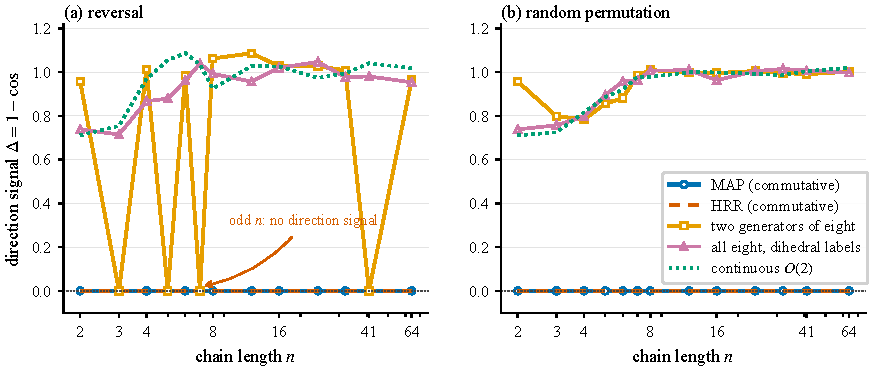
\includegraphics[width=\textwidth]{figures/fig_direction.pdf}
  \caption{Direction signal $\Delta = 1 - \cos$ against chain length, forward composition only. (a) Reversal. The commutative arms sit on zero at every length: no direction information exists for a readout to recover. The two-generator family --- the one the kernel-tier instance is built from --- alternates, dropping to exactly zero at every odd length, which is Theorem~\ref{thm:blind} as a runtime signature. (b) A mean over eight distinct non-identity reorderings. All three order-sensitive families rise together and the commutative arms stay at zero, so what the two-generator family loses at odd lengths is reversal specifically, not reordering in general.}
  \label{fig:direction}
\end{figure}

Restricting to the hop lengths that actually occur in the curriculum makes the consequence concrete, and it is a categorical split rather than a margin. Over the 33 distinct hop lengths of 1{,}200 sampled real prerequisite paths, the two commutative families carry no direction signal at 33 of 33; the two-generator family at 16 of 33, exactly the odd ones; the eight-element and continuous families at 0 of 33. Only the length distribution is taken from the curriculum --- the relations must be group elements for the algebra to apply at all --- so this is a real-length rather than a real-relation measurement, and we do not claim more. Path enumeration iterates a sorted ancestor list rather than the set the graph library returns; without that, per-process string hashing makes the sampled length multiset differ between runs, which moved this count by one when we first measured it.

\paragraph{A prediction, not a description.} The $n = 2$ value is derived rather than observed, which makes it the one number here that tests the model. For an orthogonal codebook the cosine between the two orderings reduces, per block, to $\tfrac{1}{2}\operatorname{tr}(g_1^{\mathsf{T}} g_2^{\mathsf{T}} g_1 g_2)$: half the trace of the group commutator, so $\Delta = 1 - \tfrac{1}{2}\operatorname{tr}$. In $O(2)$ the commutator is the identity exactly when both relations are rotations and is otherwise a rotation whose trace averages to zero, so a continuous family predicts $\cos = \tfrac14$; the eight-element group has $|G|$ times its five conjugacy classes, i.e.\ 40 commuting pairs of 64, the other 24 contributing $\operatorname{tr}(\texttt{Rot}^2) = -2$, again $\tfrac14$; two generators alone give $(1 + 1 - 1 - 1)/4 = 0$, i.e.\ full reversal blindness on average. Measured over 400 independent relation draws: $0.2504 \pm 0.0016$, $0.2490 \pm 0.0022$ and $-0.0053 \pm 0.0021$ respectively. The first two sit within one standard error of their predictions; the third is at $2.5$, which we report rather than round away --- the prediction there is exactly zero, so any residual is visible as a multiple of a standard error however small it is in absolute terms. (In Table~\ref{tab:reversal} one relation chain is shared across the trial batch, so the effective sample size there is the block count $D/4 = 512$ and the standard error about $0.044$, which is why its $n = 2$ column sits a few hundredths off the closed form.)

\subsection{Chain recovery survives floating point}
\label{sec:runtime}

The algebraic tier needs no measurement: \texttt{chain\_exact\_unbind} kernel-checks. The runtime tier asks whether a float32 implementation realizes it, with the curriculum DAG supplying the chain lengths --- the 56{,}224 pairs span 40 distinct hop lengths, each sampled with 200 random integer contents and 50 float32 trials, for 8{,}000 and 2{,}000 roundtrips. Every chain is heterogeneous: an independent relation at each hop, drawn i.i.d.\ from the two-element generating set of the verified family, bound forward and unbound in reverse. In the integer regime, mirroring the Lean model, recovery is exact in 200 of 200 trials at every length; exactness there is entailed by orthogonality, so it confirms the implementation matches the model rather than supplying independent evidence. The float32 measurement is the informative one: maximum absolute error grows from $2.4\times10^{-7}$ at hop 2 to $1.4\times10^{-6}$ at the longest chains, tracking accumulation of rounding across more sequential products rather than failure of the guarantee. This is \S\ref{sec:recovery} measured (Figure~\ref{fig:chain-error}) --- recovery does not degrade with $n$ the way a superposing encoding would, because there is no superposition to degrade.

\begin{figure}[t]
  \centering
  
\includegraphics[width=\textwidth]{figures/fig_chain_error.pdf}
  \caption{(a) The 56{,}224 transitive prerequisite pairs by chain length; (b) maximum absolute float32 error of the bind/unbind roundtrip against chain length. Both axes log-scaled. Pair counts peak near hop 12 and taper to the maximum observed length of 41; error grows with length while remaining bounded at $1.4\times10^{-6}$, consistent with float32 accumulation rather than algebraic failure.}
  \label{fig:chain-error}
\end{figure}


\subsection{The two encodings, and the superposition law}
\label{sec:capacity-exp}

\texttt{chain\_length\_separation.py} measures both encodings --- role-filler and composition --- on the identical operator implementation, $D = 2{,}048$ and content codebook, in top-1 retrieval accuracy. One asymmetry bounds what the comparison shows: the two do not store the same amount. Role-filler holds $n$ key--value bindings and offers random access to any slot; composition holds one content and requires the whole relation sequence to unwind it. At $T = 1$ exactness follows from orthogonality of the sampler, so composition's flat line is entailed rather than measured, and the informative content is the \emph{shape} of the role-filler curve.

Composition recovers exactly at every measured length, accuracy 1.0 from $n = 2$ to $n = 150$ for both the verified operator and MAP, while role-filler encoding of the identical chains degrades as the superposition argument predicts: 98.1\% at $n = 64$, 84.6\% at $n = 100$, 59\% at $n = 150$, with MAP and HRR collapsing on the same curve (Figure~\ref{fig:separation}). Two things follow. Role-filler retrieval stays at 1.0 through $n = 41$, so the algebraic crosstalk of \S\ref{sec:superposition} is \emph{not} the same thing as retrieval failure --- a contaminated vector can still win nearest-neighbour lookup against a 2{,}000-entry codebook. And composition being exact for MAP as well is the runtime face of \S\ref{sec:recovery}: recovery needs a left inverse, which MAP has. HRR is the exception, collapsing to near-chance by $n = 24$; that is not a counterexample to composition never crosstalking but what happens when composition is attempted with an operator whose unbind is only approximate, since HRR uses the complex conjugate as a stand-in for an exact inverse and \S\ref{sec:pair-tiers} measures its single-hop fp32 fidelity at 0.7084. \texttt{chain\_exact\_unbind} is unconditional \emph{given} Axiom 3, and HRR does not satisfy that axiom.

\begin{figure}[t]
  \centering
  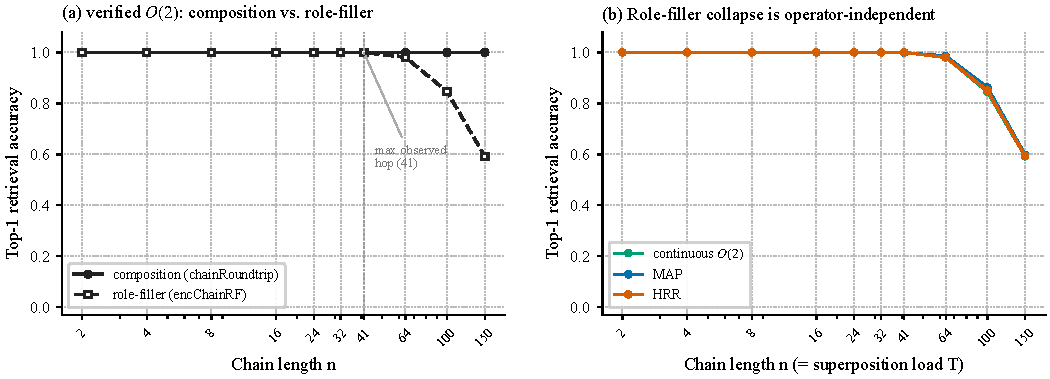
\includegraphics[width=\textwidth]{figures/fig_separation.pdf}
  \caption{Top-1 retrieval accuracy versus chain length $n$, identical operator implementation, dimension and codebook for both encodings. (a) Composition is exact at every measured length; role-filler encoding of the identical chains degrades once $n$ exceeds roughly the codebook-relative capacity. The dotted line marks the longest hop length observed in the curriculum graph (41). (b) The role-filler degradation curve is indistinguishable across MAP, HRR and the verified operator.}
  \label{fig:separation}
\end{figure}

A controlled sweep gives the law that curve obeys, and we fit its exponent rather than assume it. The sweep varies superposition load $T$ and dimension $D$, drawing keys \emph{without replacement} from a codebook of $K = 2{,}000 \gg \max T$, so top-1 accuracy is not capped by key collisions unrelated to crosstalk. Over 72 $(\text{operator}, T, D)$ points, accuracy is a logistic function of $z = \sqrt{D/T}$ with $R^2 = 0.99$ against $R^2 = 0.52$ for a model linear in the same $z$ --- but both use the same $z$, so that comparison tests functional form and says nothing about the exponent. \citet{frady2017superposition} derive signal-to-noise $\sqrt{N/M}$ from a Gaussian-tail argument, which predicts that the \emph{probit} of accuracy is linear in the SNR, and fitting in probit space turns the exponent into a least-squares problem. On the unsaturated cells the best exponent in $\operatorname{probit}(\mathrm{acc}) \sim a\,(D/T)^{\alpha} + b$ is $\alpha = 0.48$ with $R^2 = 0.9998$ against a predicted $0.5$; freeing the two exponents separately in $D^{p}/T^{q}$ gives $p = q = 0.48$, confirming independently that $D$ and $T$ enter only through their ratio. We therefore state the relation as a test rather than a corroboration, with one caveat: the verified operator's codebook is orthogonal by construction and MAP's bipolar, so neither is the i.i.d.\ random codebook the derivation assumes. The consequence cuts against our own operator --- if retrieval from superposition is governed by $\sqrt{D/T}$ regardless of the binding algebra, no choice of operator can buy capacity.


\subsection{Where the operator does not matter, as predicted}
\label{sec:pair-tiers}

Remark~\ref{rem:predictions}, which follows from \S\ref{sec:h0}, predicts that on any tier reducing to pair-level order recovery, commutative and non-VSA controls should match the verified operator. Five independent settings do. We report them as consistent with the prediction rather than as confirming it --- the theorem is existential, and \S\ref{sec:threats} gives a competing explanation the same data admits --- but the direction of the evidence is worth stating: a theory that predicts its own null results is doing more work than one that only predicts wins.

\emph{Two learned probe tiers.} The verified operator attains 85.6\%/94.8\%/98.7\% across hop strata transductively (93.0\% overall) and 69.2\%/81.8\%/92.6\% inductively (81.2\% unweighted, 87.1\% weighted). A \texttt{concat-MLP} probe --- order-sensitive but with no binding operator and no algebraic guarantee --- matches it on both tiers, at 80.6\%/92.5\%/98.9\% and 68.2\%/79.0\%/93.4\%, with overlapping bootstrap intervals at all six strata (Table~\ref{tab:controls}). These tiers establish that the content representation supports direction recovery at the reported rates, and establish nothing about the operator.

\emph{Two commutative substitutions.} MAP's bipolar codebook makes the nested-bind architecture used by every VSA arm exactly floating-point order-invariant, so forward and reverse scores are bit-identical on every pair; shown as ``tie''. HRR's convolution is order-invariant only in exact arithmetic, so margin-ranking training exploits residual floating-point asymmetry --- its strict accuracy of 13.2--14.1\% is a tie-break artifact, and we report the tie-broken value. Neither shows that commutative binding cannot encode pair order: Theorem~\ref{thm:h0} is about the \emph{role-filler} construction, and this architecture nests bind at the outer level as $\texttt{bind}(\texttt{bind}(u, r_P), \texttt{bind}(v, r_A))$, which collapses to a symmetric ring product for any commutative associative operator. Re-running the identical protocol with the literal role-filler construction (\texttt{src/eduhdc/\allowbreak prereq\_role\_filler\_probe.py}) confirms the theorem: MAP attains 80.5\%/91.7\%/98.5\% transductively and 68.8\%/77.9\%/93.5\% inductively against the verified operator's 78.1\%/90.0\%/98.0\% and 67.1\%/77.9\%/92.3\%, matching or exceeding it at every stratum of both tiers, and HRR does likewise at 81.7\%/92.4\%/98.8\% transductively. The verified operator scores \emph{lower} under role-filler encoding than under nested bind, so the arms converge partly because it gives up an architectural advantage.

\begin{table}[t]
\centering
\caption{Direction accuracy with operator controls, 10 seeds, percentile bootstrap 95\% intervals over seeds, each arm early-stopped on a per-hop-stratum validation split. The non-VSA control's interval overlaps the verified operator's at all six cells. Bold marks the highest value in a column; it is not marked where a difference lies inside the intervals. $^\dagger$ tie-broken.}
\label{tab:controls}
\small
\begin{tabular}{lcccccc}
\toprule
& \multicolumn{3}{c}{Transductive (pair held out)} & \multicolumn{3}{c}{Inductive (node held out)} \\
\cmidrule(lr){2-4}\cmidrule(lr){5-7}
Arm & hop 2--3 & hop 4--6 & hop 7+ & hop 2--3 & hop 4--6 & hop 7+ \\
\midrule
Verified $O(2)$ family        & 85.6\% & 94.8\% & 98.7\% & 69.2\% & 81.8\% & 92.6\% \\
MAP (commutative)             & tie    & tie    & tie    & tie    & tie    & tie \\
HRR (commutative)             & 49.8\%$^\dagger$ & 49.9\%$^\dagger$ & 49.4\%$^\dagger$ & 50.1\%$^\dagger$ & 49.3\%$^\dagger$ & 49.8\%$^\dagger$ \\
\texttt{concat-MLP} (non-VSA) & 80.6\% & 92.5\% & \textbf{98.9\%} & 68.2\% & 79.0\% & \textbf{93.4\%} \\
\bottomrule
\end{tabular}
\end{table}

\emph{A knowledge-tracing benchmark, and a frozen-codebook ablation.} On ASSISTments 2012--2013 (5-fold, 5{,}000 students, a pyKT-standard protocol \citep{liu2022pykt}), substituting the verified operator as the per-step bind/unbind memory update gives 0.7152 $\pm$ 0.0034 AUC against DKT's 0.7109 $\pm$ 0.0030 \citep{piech2015deep} ($+0.0043$, $p = 0.015$, $d_z = 1.83$), reversing sign under a 10-fold, 8{,}000-student check at 0.7190 against 0.7206 ($-0.0016$, $p = 0.0057$, $d_z = -1.14$); significance in one direction at one sample size and the opposite at a larger one is evidence against a stable ordering, so we report parity. The commutative substitutions are competitive at both sizes (MAP 0.7155 and 0.7173; HRR 0.7133 at 5{,}000, omitted at 10-fold for compute cost), the verified operator's margin over MAP ($+0.0017$ at 8{,}000, $p = 1.9\times10^{-4}$; $-0.0003$ at 5{,}000, $p = 0.74$) is smaller than either arm's fold-to-fold standard deviation, and the other baselines trail: SAKT 0.6856/0.6991 \citep{pandey2019sakt}, simpleKT 0.6856/0.6978 \citep{liu2023simplekt}, AKT 0.6998/0.7056 \citep{ghosh2020akt}. Two costs belong beside that: of the readout's seven features only two come from the VSA, and zeroing them drops AUC from 0.7159 to 0.6891 ($+0.0268$, $p = 1.2\times10^{-7}$) but refilling the slots with two cheap, strictly causal, non-VSA statistics recovers 73\% of the gap, leaving $+0.0072$ ($p = 6.6\times10^{-5}$) attributable to what bind and unbind compute; and the architecture costs 537{,}415 parameters against DKT's 166{,}276, at 0.406\,ms per student against 0.067\,ms. Separately, a frozen-codebook variant with 828 trainable parameters --- 197 fewer than DKT --- still reaches parity with DKT, which is an architectural property rather than an algebraic one, since frozen-codebook MAP attains equal or higher AUC.

\paragraph{What the operator does buy at runtime.} A precision study on randomly generated 2{,}048-dimensional hypervectors measures cosine similarity between true and quantized unbinding across fp32, bf16, fp16 and int8. The verified operator attains exactly 1.0 at fp32 --- entailed by the orthogonal sampler, so it confirms only that the implementation contains no defect --- while HRR, a circular-convolution operator outside the specification, attains only 0.7084 even at fp32: exact unbinding is not generic to VSA binding. The verified operator stays above 0.9998 under int8, so the fixed-width state \S\ref{sec:superposition} secures algebraically survives 8-bit quantization.


\section{What Is Proved, What Is Measured}
\label{sec:proved-measured}

Scope conditions on the proved rows follow in \S\ref{sec:limitations}; conditions bounding how far the measured rows generalize follow in \S\ref{sec:threats}; the open problems each leaves are collected in \S\ref{sec:outlook}.

\begin{table}[h]
\centering
\small
\begin{tabular}{p{0.50\textwidth}p{0.42\textwidth}}
\toprule
Claim & Evidence \\
\midrule
No abelian-label family can satisfy Axiom 2, for any carrier & Kernel-checked (Theorem~\ref{thm:abelian}); necessary, not sufficient; assumes closure under composition \\
An abelian-label family cannot distinguish \emph{any} reordering & Kernel-checked at every length, no invertibility assumed (Theorem~\ref{thm:perm}) \\
Axiom 2 yields two orderings that differ, at every length & Kernel-checked (Theorem~\ref{thm:order-general}); a witness pair per length, not every pair \\
Axiom 2 does \emph{not} yield reversal discrimination & Kernel-checked counterexample at length three in our own verified family (Theorem~\ref{thm:blind}); odd-length pattern verified exhaustively, not proved \\
A family exposing the whole label algebra does & Kernel-checked at every length (Theorem~\ref{thm:d4}) \\
\midrule
Commutative arms blind to reversal and permutation at cosine 1.0 & Measured, 13 lengths, forward composition (\S\ref{sec:order-exp}) \\
Two-generator family blind at odd lengths only; on real hop lengths, 16 of 33 & Measured (\S\ref{sec:order-exp}) \\
$n=2$ cosine equals half the mean commutator trace & Derived and confirmed to three decimals (closed form, \S\ref{sec:order-exp}) \\
Non-VSA and commutative controls match at pair level, including knowledge tracing & Measured, 5 settings; consistent with a competing explanation (\S\ref{sec:threats}) \\
\bottomrule
\end{tabular}
\end{table}

\section{Limitations}
\label{sec:limitations}

\begin{enumerate}
\item \textbf{The criterion is necessary, not sufficient, and assumes closure.} Theorem~\ref{thm:abelian} rules families out; it does not admit them, since Axioms 1 and 3 separately demand linearity and invertible action. It also constrains only families closed under composition --- the \texttt{ops} field of \texttt{PedagogicalVSA} does not require closure, so a family assembled from unrelated functions is outside its reach. The two concrete impossibility theorems are narrower still: they rule out families drawn \emph{entirely} from the named construction, not mixed families containing one order-sensitive pair. The strengthened axiom closing that loophole is discharged only for the integer instances.
\item \textbf{Direction is diagnosed, not characterized.} We exhibit one family that satisfies Axiom 2 and is reversal-blind at odd lengths, and one that is not blind at any length. We give no general condition on a generating set under which reversal is distinguishable at every length, and the odd-length pattern for the two-generator family is verified by exhaustive search rather than proved for all odd $n$.
\item \textbf{The positive results are witnesses, not universals.} Theorem~\ref{thm:order-general} exhibits one distinguishable pair of orderings per length rather than characterizing which orderings a family separates; Theorem~\ref{thm:h0} does not assert that every commutative encoding distinguishes order; and the crosstalk witness shows naive recovery \emph{can} fail at any length, not that it fails for every choice of contents and roles, nor that contamination worsens with length --- the padding that extends it is inert, so its effective load is 2 at every $n$.
\item \textbf{The integer instances are not independent.} In dimension two the integer orthogonal group and the signed-permutation group coincide, so those two are generating sets for one eight-element group. \texttt{d4VSA} is a third instance over the same group but with a distinct label type; a structurally independent permutation family needs $S_3$ and a $3\times3$ carrier we do not formalize.
\item \textbf{The specification is deliberately thin.} \texttt{bundle} carries no axioms of its own, so \texttt{PedagogicalVSA} is not a reusable algebraic structure in the Mathlib sense. \S\ref{sec:pairs} turns that into a result, but a reader adopting the specification should know it permits non-surjective binding and unconstrained superposition.
\item \textbf{Invertibility is assumed, and real curricula violate it.} \texttt{exact\_unbind\_ax} presupposes every relation is invertible, and \citet{yang2022knowledgebra} show that must break for knowledge graphs --- relations form a semigroup whose non-invertible elements are exactly the N-to-1 case --- with \citet{chaki2026kraus} reaching the same place by rank. We do not repair the specification but we measure the damage: dropping \texttt{inv} and \texttt{exact\_unbind\_ax} leaves composition intact (\texttt{chainApply\_bundle\_distrib} needs no invertibility) and leaves Theorem~\ref{thm:abelian} untouched, so commutative operators stay excluded from the weakened specification too, while exact recovery provably does not survive: \texttt{nonInjMonoid} satisfies both remaining axioms with a rank-one projection, and \texttt{nonInjMonoid\_not\_from\_VSA} shows no \texttt{PedagogicalVSA} can have its operators. Relatedly, the recovery guarantee certifies only the full roundtrip on a known intermediate path: recovering state part-way along a chain, and predicting a relation with no connecting path, are both outside it.
\end{enumerate}


\section{Threats to Validity}
\label{sec:threats}

\paragraph{Internal.} Every knowledge-tracing baseline runs at embedding width 64 while VSA arms use 2{,}048-dimensional codebooks; AKT in particular is configured well below its authors' width, the likely reason it trails DKT here when published comparisons place it above. The baseline column should read as same-budget-per-baseline, not each model's best. DKT's learning rate was not swept on ASSISTments; our one sweep, on a different dataset, found a higher value better, so DKT may be understated. VSA arms train at a larger learning rate than the baselines, a gap not swept jointly.

\paragraph{Construct.} The learned tiers use one probe architecture per arm, so an accuracy measures that architecture's use of an operator's output, not an operator ceiling --- the role-filler rerun moves the verified operator by up to 7.4 points at one stratum, which bounds how much any single number says. Content embeddings are sentence encodings of exercise \emph{names}, with no difficulty or stage metadata leaked; nevertheless topic and depth are recoverable from a name, and no ablation removes that signal before probing. This is a competing explanation for all five pair-level matches: if the probes recover curriculum depth from names rather than relational structure, every operator would match regardless of Theorem~\ref{thm:h0}, and we report the matches as consistent with the theorem rather than as confirming it. The confound is specific to the learned tiers. \S\ref{sec:order-exp} has a different limit rather than the same one: nothing is trained and no readout is involved, but its relations are drawn from each operator's group and its contents at random, with only the hop-length distribution coming from the curriculum. It therefore measures what the algebra contains at real curriculum lengths, not what a learned system would extract from real curriculum relations.

\paragraph{External.} Evaluation is restricted to a single curriculum graph, whose 832 nodes fall into 70 weakly connected components with 60 isolated nodes; the largest holds 740 nodes and 97\% of transitive pairs. The hop distribution is heavily right-skewed --- hop 2--3 is 4.6\% of pairs, hop 4--6 is 10.2\%, hop 7+ is 85.2\% --- which is what makes the path-level premise operative and simultaneously means any stratum-weighted statistic is dominated by hop 7+, so we report unweighted figures alongside weighted ones. Separately, training the verified operator only on a small, independently sourced expert-annotated set (615 binary and 75 directionally-asymmetric pairs from \citet{chang2015modeling}) and evaluating zero-shot on curriculum-derived pairs gives 48.4\% direction accuracy. Checking the convention by hand against both sources did reveal a systematic reversal --- 81\% of the annotation pairs that resolve to a direction in the DAG run opposite to it --- but not one that explains the number, since flipping every annotation direction recovers only to 51.94\% (pooled Wilson 95\% CI [51.25, 52.63]). The residual is cross-source disagreement driven by coverage: expert annotations are all but confined to short hops while the test set is dominated by hop 7+. It is a labelling and coverage difference, not a verdict on any binding algebra, and nothing here proposes a learned component to compensate for it.

\paragraph{Statistical.} Every bootstrap interval is over 10 seeds, enough to detect the reported effects but not to rule out smaller ones; at 10 seeds a nominal 95\% percentile interval has actual coverage below 95\%, so intervals read as indicative and overlap as absence of evidence for a difference, not evidence of equality. The per-stratum validation split is drawn with a seed depending on arm index, so each arm early-stops on a slightly different holdout. Paired $t$-tests over cross-validation folds treat fold AUCs as independent when consecutive folds share most training data, so variance is understated \citep{nadeau2003inference}; we report them by convention, and the sign flip rather than either $p$-value carries the parity reading. No multiplicity correction is applied. The chain-length separation reports one deterministic draw of 30 trials per point, and in Table~\ref{tab:reversal} one relation chain is shared across the trial batch, so the effective sample size there is the block count; the closed-form comparison in \S\ref{sec:order-exp} redraws relations and is the estimate to cite.


\section{Outlook}
\label{sec:outlook}

The counterexample is the least finished result here and the first target. We show that Axiom 2 does not deliver reversal discrimination and that exposing a whole label algebra does, for one group. What is missing is a condition on a generating set of a non-abelian group under which some chain of every length is distinguishable from its reverse. The two-generator dihedral case suggests the obstruction is a parity invariant of words over the generating set, which would make the condition checkable rather than a matter of exhaustive search. A second quantifier gap sits on the crosstalk side: the witness is contaminated at every length by a padding argument whose extra terms are inert, and a statement covering every choice of contents and roles needs an argument that crosstalk cancellation is algebraically impossible.

The criterion itself invites mechanization. Adding an operator to the kernel tier currently means defining it on the carrier, discharging orthogonality and bundle distributivity, exhibiting a non-commuting intra-family pair, and packaging the instance --- reachable with a few weeks' Lean 4 experience, since every obligation reduces to linear integer arithmetic. A construction taking a label algebra and a linearity witness to an instance would turn Table~\ref{tab:criterion} from a list into a decision procedure.

The gap that matters most for practice is an evaluation whose \emph{learned} task exercises the chain-level results. Every learned tier here reduces to pair-level order recovery, which \S\ref{sec:pairs} says cannot separate operators, and \S\ref{sec:order-exp} shows the algebra contains order information a commutative operator lacks --- but without a learned component anywhere. Closing that needs a task where a model must commit to a traversal direction over a path it has not seen, and where the operator rather than the content embedding is the only thing that could supply it.


\section{Conclusion}
\label{sec:conclusion}

We asked what non-commutative binding is for, and found the field's one-word answer covering four requirements with different prices. Ordered-pair representation needs two distinct roles and nothing more: a role-filler encoding built from two \emph{commutative} roles, with invertible bipolar codebook entries, already distinguishes $(u,v)$ from $(v,u)$, and on real curriculum data a commutative operator given that construction matches the verified one at every stratum of two tiers. Recovery of a composed chain needs a left inverse and nothing more; a commutative operator has one and achieves exact recovery to $n = 150$. Reordering is where the order axiom is both necessary and sufficient: abelian labels make every permutation of a chain the same map at every length, and conversely the axiom yields two orderings that differ at every length.

Direction is the fourth, and it is where a natural reading of the axiom fails. Telling a traversal from its reverse is one particular reordering, and the axiom does not deliver it: our own verified family satisfies it and is provably blind to reversal at length three, and at every odd length by exhaustive search, because it exposes two of its group's eight elements. Exposing all eight repairs it at every length. Measured on the hop lengths a real curriculum contains, the two commutative arms are blind at 33 of 33 lengths, the two-generator family at exactly the 16 odd ones, and the family exposing all eight at none --- the one categorical separation in this paper, against parity everywhere else.

That pattern is the point rather than an apology for it. Every setting where the arms tie is a setting the pair-level theorem predicts will tie, and a theory that predicts its own null results is doing more work than one that only predicts wins. The criterion is what we expect to outlive the particular operator: order sensitivity lives in the label algebra, so an abelian one is excluded without measurement and a non-abelian one is a candidate without a fresh instance proof. But a candidate is all it is, and Remark~\ref{rem:coverage} states how far we take that. Non-commutativity is necessary for order and not sufficient for direction, and what closes the gap is not a stronger axiom but a family that uses more of the algebra it is drawn from.


\section*{Code and Data Availability}

All Lean 4 proof scripts, Python evaluation code, and result JSON files underlying these results are available at \url{https://github.com/linhtvu11/eduhdc}; a versioned release tag timestamps the exact code state corresponding to this preprint. The Junyi Academy curriculum graph and the \citet{chang2015modeling} expert prerequisite annotations are third-party datasets, obtained under their original terms of release; ASSISTments 2012--2013 is likewise third-party, used under its standard research-use terms.

\bibliographystyle{plainnat}
\bibliography{references}

\end{document}
